\section{Auswertung}
\label{sec:Auswertung}

\subsection{Zeitabhängigkeit der Amplitude}

Die gemessenen Maxima bei einer gedämpften Schwingung sind 
in Tabelle \ref{tab:Messdaten1} zu sehen. 

\begin{table}
\centering
\caption{Messdaten der Maxima der Amplitude}
\label{tab:Messdaten1}
\sisetup{table-format=2.1}
\begin{tabular}{c c}
\toprule
$U \,/\, \si{\volt}$ & $s \,/\, \si{\micro\second}$\\
\midrule
1,74 &   0,0\\
1,44 &  29,6\\
1,20 &  58,8\\
1,10 &  88,2\\
0,84 & 117,2\\
0,68 & 147,2\\
0,56 & 177,2\\
0,46 & 206,2\\
0,38 & 235,2\\
0,30 & 265,2\\
0,22 & 294,2\\ 
0,16 & 324,2\\
0,14 & 353,2\\
0,10 & 382,2\\
0,06 & 412,2\\
0,02 & 441,2\\
0,00 & 471,2\\
\bottomrule
\end{tabular}
\end{table} 

Die Ausgleichsrechnung wird mit der Funktion 

\begin{equation*}
A = A_0 \cdot e^{-2\pi\mu t}
\end{equation*}

durchgeführt. Das Ergebnis ist in Abbildung \ref{fig:gedämpft} zu sehen. 

\begin{figure}
  \centering
  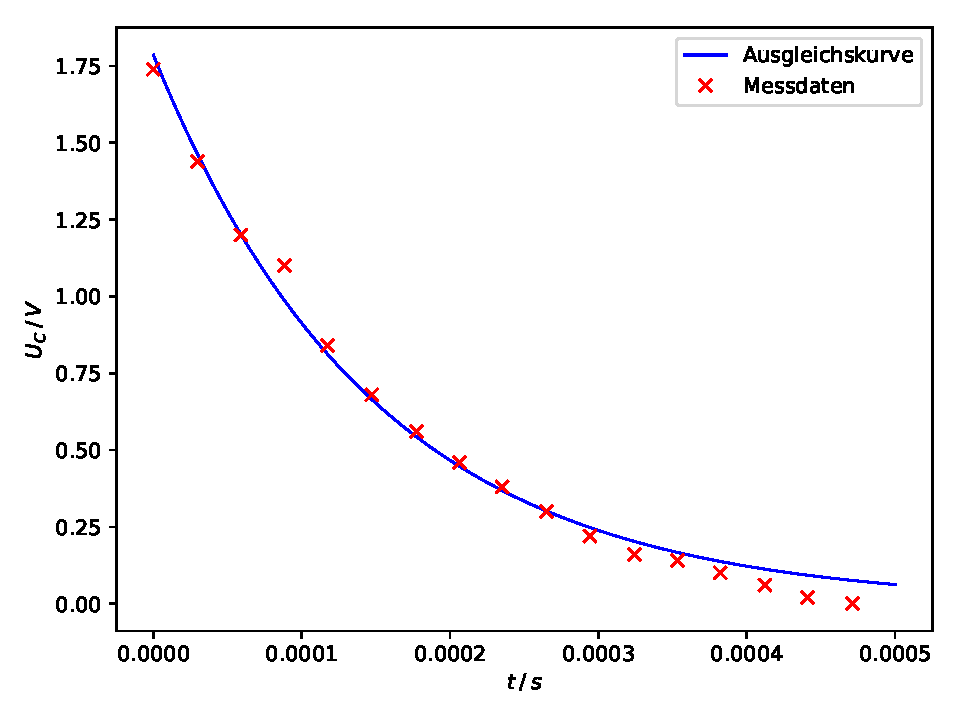
\includegraphics[scale=0.8]{content/plot1.pdf}
  \caption{Exponentielle Regression der Amplitude}
  \label{fig:gedämpft}
\end{figure}

Mittels python ergeben sich die Regressionsparamter zu: 

\begin{align*}
A_0 &= \SI{1.785+-0.036}{\volt},\\
\mu &= \SI{1068.421+-34.320}{\per\second}.
\end{align*}

Mit Formel... lässt sich nun der effiktive Widerstand berechnen.

\begin{equation*}
R_\text{eff} = 4\pi L\mu = \SI{136+-4}{\ohm}
\end{equation*}

Der Fehler ergibt sich dabei durch die Gaußsche Fehlerfortpflanzung zu: 

\begin{equation*}
\symup{\Delta} R_\text{eff} = \sqrt{\left(\frac{\symup{d}R_\text{eff}}{\symup{d}L}\right)²\cdot (\symup{\Delta}L)² +
\left(\frac{\symup{d}R_\text{eff}}{\symup{d}\mu}\right)²\cdot (\symup{\Delta}\mu)²}.
\end{equation*}

Weiterhin wird die Abklingdauer mit Formel... berechnet und 
es ergibt sich:

\begin{equation*}
T_\text{ex} = \frac{1}{2\pi\mu} = \SI{0.149+-0.005e-3}{\second}.
\end{equation*}

Der Fehler ergibt sich hierbei zu: 

\begin{equation*}
\symup{\Delta} T_\text{ex} = \sqrt{\left(\frac{\symup{d}T_\text{ex}}{\symup{d}\mu}\right)²\cdot (\symup{\Delta}\mu)²}.
\end{equation*}

\subsection{Bestimmung des Dämpfungswiderstandes}

Hier wurde der aperiodische Grenzfall untersucht. Dabei wurde der
Dämpfungswiderstand zu 

\begin{equation*}
R_\text{ap} = \SI{3520+-50}{\ohm}
\end{equation*}

bestimmt.
Der theoretische Wert von $R_\text{ap}$ kann mit Formel \eqref{eqn:apth} bestimmt 
werden: 

\begin{equation*}
R_\text{ap,theo} = \SI{4390+-9}{\ohm}.
\end{equation*}

Der Fehler berechnet sich über die Gaußsche Fehlerfortpflanzung: 

\begin{equation*}
\symup{\Delta} R_\text{ap,theo} = \sqrt{\left(\frac{\symup{d}R_\text{ap}}{\symup{d}L}\right)²\cdot (\symup{\Delta}L)² +
\left(\frac{\symup{d}R_\text{ap}}{\symup{d}C}\right)²\cdot (\symup{\Delta}C)²}.
\end{equation*}

\subsection{Frequenzabhängigkeit der Kondensatorspannung}

Die gemessenene Kondensatorspannung $U_C$ und die zugehörige Frequenz $f$, sowie
die Erregerspannung $U_0$ sind in Tabelle \ref{tab:Messdaten2} aufgeführt. 

\begin{table}
  \centering
  \caption{Messdaten der frequenzabhängigen Kondensatorspannung}
  \label{tab:Messdaten2}
  \sisetup{table-format=2.1}
  \begin{tabular}{c c c}
  \toprule
  $f \,/\, \si{\kilo\hertz}$ & $U_C \,/\, \si{\volt}$ & $U \,/\, \si{\volt}$ \\
  \midrule
  09 & 1,08 & 0,56\\
  11 & 1,12 & 0,56\\
  13 & 1,16 & 0,56\\
  15 & 1,22 & 0,54\\
  17 & 1,30 & 0,56\\
  19 & 1,40 & 0,54\\
  21 & 1,56 & 0,56\\
  23 & 1,72 & 0,56\\
  25 & 1,96 & 0,56\\
  27 & 2,36 & 1,04\\
  29 & 2,84 & 0,96\\
  30 & 3,08 & 1,00\\
  31 & 3,40 & 1,00\\
  32 & 3,64 & 1,00\\
  33 & 3,72 & 1,00\\
  34 & 3,76 & 1,00\\
  35 & 3,56 & 1,00\\
  36 & 3,24 & 1,00\\
  37 & 2,92 & 1,00\\
  38 & 2,60 & 1,00\\
  39 & 2,28 & 1,00\\
  41 & 1,80 & 1,00\\
  43 & 1,48 & 1,04\\
  45 & 1,20 & 1,04\\
  47 & 0,98 & 0,52\\
  49 & 0,84 & 0,52\\
  51 & 0,74 & 0,52\\
  53 & 0,64 & 0,52\\
  55 & 0,59 & 0,21\\
  57 & 0,54 & 0,21\\
  59 & 0,49 & 0,21\\
  \bottomrule
  \end{tabular}
  \end{table} 

Es wird $\frac{U_C}{U_0}$ in Abbildung ... gegen die Frequenz aufgetragen. 

\begin{figure}
  \centering
  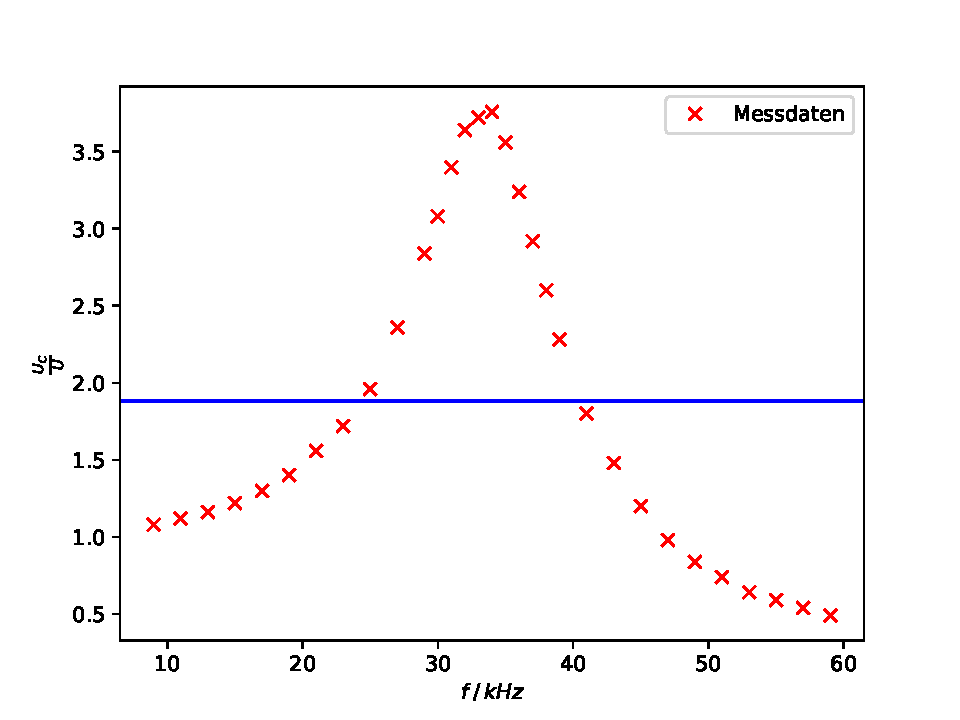
\includegraphics[scale=0.8]{content/plot2.pdf}
  \caption{Resonanzkurve}
  \label{fig:resonanz}
\end{figure}

Die experimentelle Resonanzüberhöhung wird aus der Abbildung als 

\begin{equation*}
q_\text{ex} = \num{3.76}
\end{equation*}

Der theoretische Wert der Resonanzüberhöhung berechnet sich über die Formel 
... zu: 

\begin{equation*}
q_\text{theo} = \frac{\sqrt{L}}{R\sqrt{C}} = \num{4.309+-0.010}.
\end{equation*}

Der Fehler ergibt sich dabei durch die Gaußsche Fehlerfortpflanzung: 

\begin{equation*}
\symup{\Delta}q_\text{theo} = \sqrt{\left(\frac{\symup{d}q}{\symup{d}R}\right)²\cdot(\symup{\Delta}R)² +
\left(\frac{\symup{d}q}{\symup{d}L}\right)²\cdot(\symup{\Delta}L)²+
\left(\frac{\symup{d}q}{\symup{d}C}\right)²\cdot(\symup{\Delta}C)²}. 
\end{equation*}

Der experimentelle Wert der Halbwertsbreite $b$ wird aus der Abbildung als 

\begin{equation*}
b_\text{ex} = \omega _+ - \omega _- = \SI{38}{\kilo\hertz} - \SI{28}{\kilo\hertz} = \SI{10}{\kilo\hertz} 
\end{equation*}

abgelesen.
Der theoretische Wert für die Breite liegt jedoch bei 

\begin{equation*}
b_\text{theo} = \frac{R}{2\pi L} = \SI{8.021+-0.025}{\kilo\hertz}.
\end{equation*}

Dabei ergibt sich der Fehler mit: 

\begin{equation*}
\symup{\Delta}b_\text{theo} = \sqrt{\left(\frac{\symup{d}b}{\symup{d}R}\right)²\cdot(\symup{\Delta}R)² +
\left(\frac{\symup{d}q}{\symup{d}L}\right)²\cdot(\symup{\Delta}L)²}.
\end{equation*}

\subsection{Frequenzabhängigkeit der Phasenverschiebung}

Die Messwerte der Zeitdifferenz $\symup{\Delta} t$ in Abhängigkeit der Frequenz $f$, sowie die daraus errechnete
Phasendifferenz

\begin{equation}
  \phi = 2 \pi - \frac{\Delta t}{f} \cdot 2 \pi
  \label{eqn:Diff}
\end{equation}

sind in Tabelle \ref{tab:Messdaten3} aufgelistet. Die Subtraktion von $2 \pi$ in \eqref{eqn:Diff} hängt dabei mit der 
Messdurchführung zusammen, d.h. $\symup{\Delta} t$ wurde zuzüglich einer Periode gemessen. 


\begin{table}
  \centering
  \caption{Messdaten der frequenzabhängigen Phasendifferenz}
  \label{tab:Messdaten3}
  \sisetup{table-format=2.1}
  \begin{tabular}{c c c}
  \toprule
  $f \,/\, \si{\kilo\hertz}$ & $\symup{\Delta} t \,/\, \si{\micro\second}$ & $\Phi \,\, \text{in rad} $ \\
  \midrule
09 & 107,0 & 0.232 \\
11 & 088,0 & 0.201 \\
13 & 075,0 & 0.157 \\
15 & 065,2 & 0.138 \\
17 & 056,8 & 0.216 \\
19 & 050,4 & 0.266 \\
21 & 045,6 & 0.266 \\
23 & 041,2 & 0.329 \\
25 & 037,6 & 0.376 \\
27 & 034,0 & 0.515 \\
29 & 031,2 & 0.598 \\
30 & 029,2 & 0.779 \\
31 & 027,6 & 0.907 \\
32 & 025,6 & 1.136 \\
33 & 024,0 & 1.307 \\
34 & 022,0 & 1.583 \\
35 & 020,4 & 1.797 \\
36 & 019,2 & 1.940 \\
37 & 018,0 & 2.099 \\
38 & 016,4 & 2.368 \\
39 & 016,0 & 2.362 \\
41 & 014,4 & 2.574 \\
43 & 013,6 & 2.609 \\
45 & 012,8 & 2.664 \\
47 & 011,6 & 2.858 \\
49 & 011,2 & 2.835 \\
51 & 010,8 & 2.822 \\
53 & 010,4 & 2.820 \\
55 & 009,6 & 2.966 \\
57 & 009,2 & 2.988 \\
59 & 008,8 & 3.021 \\
  \bottomrule
  \end{tabular}
  \end{table} 

  In Abbildung \ref{fig:phase} sind die Phasendifferenz gegen die Frequenz aufgetragen und markierende Geraden für Phasen von
  $\frac{\pi}{4}$, $\frac{3 \pi}{4}$ und $\frac{\pi}{2}$,für welche die Frequenzen $f_1$, $f_2$ und $f_\text{res}$ (Resonanzfrequenz)
  ablesbar sind, eingezeichnet.

  \begin{figure}
    \centering
    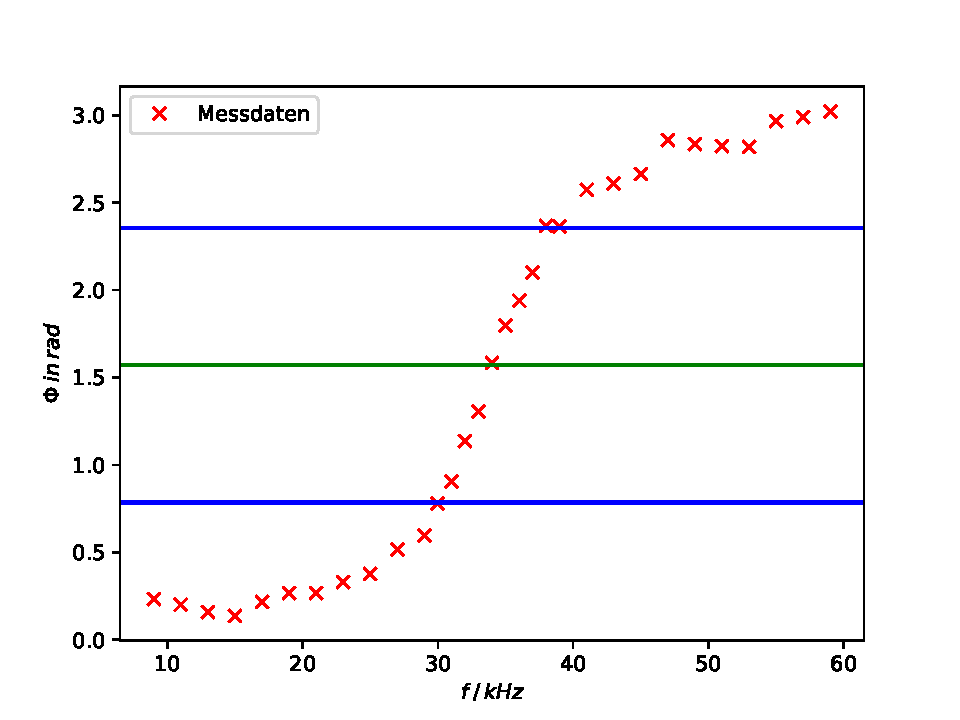
\includegraphics[scale=0.8]{content/plot3.pdf}
    \caption{Phasendifferenz}
    \label{fig:phase}
  \end{figure}

  Die abgelesenen Frequenzen sind somit:

  \begin{align*}
    f_{1,\text{ex}} &= \SI{30}{\kilo\hertz} \\
    f_{2,\text{ex}} &= \SI{38}{\kilo\hertz} \\
    f_\text{res,ex} &= \SI{34}{\kilo\hertz} \; .
  \end{align*}

  Die nach den Formeln \eqref{eqn:f12} und \eqref{eqn:fres} berechneten Frequenzen sind:

  \begin{align*}
    f_1 &= \SI{30.78 +- 0.006}{\kilo\hertz} \\
    f_2 &= \SI{38.80 +- 0.008}{\kilo\hertz} \\
    f_\text{res} &= \SI{34.09 +- 0.007}{\kilo\hertz} \; .
  \end{align*}

  Dabei berechnen sich deren Fehler nach

  \begin{align*}
    \symup{\Delta}f_{1\text{,}2} &= \sqrt{\left(\frac{\symup{d}f_{1\text{,}2}}{\symup{d}L}\right)²\cdot(\symup{\Delta}L)² +
    \left(\frac{\symup{d}f_{1\text{,}2}}{\symup{d}R}\right)²\cdot(\symup{\Delta}R)² +
    \left(\frac{\symup{d}f_{1\text{,}2}}{\symup{d}C}\right)²\cdot(\symup{\Delta}C)²} \\
    \symup{\Delta}f_\text{res} &= \sqrt{\left(\frac{\symup{d}f_\text{res}}{\symup{d}L}\right)²\cdot(\symup{\Delta}L)² +
    \left(\frac{\symup{d}f_\text{res}}{\symup{d}R}\right)²\cdot(\symup{\Delta}R)² +
    \left(\frac{\symup{d}f_\text{res}}{\symup{d}C}\right)²\cdot(\symup{\Delta}C)²} \; .
  \end{align*}